\documentclass[tikz]{standalone}
\usepackage{amsmath}
\usepackage{amssymb}
\usepackage{amsfonts}
\usepackage{tikz}
\usetikzlibrary{calc}

\thispagestyle{empty}
\begin{document}
 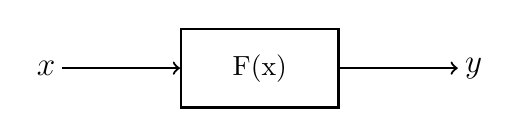
\begin{tikzpicture}[thick]

            % Function block
            \node[draw, rectangle, minimum width=2cm, minimum height=1cm] (block) at (0,0) {F(x)}; 
            
            % Input arrow 
            \coordinate (instart) at ($(block.west)+(-1.5,0)$);
            \coordinate (inmid) at ($(block.west)+(-0.75,0)$);
            \draw[->] (instart) -- (block.west);
          
            % Output arrow 
            \coordinate (outend) at ($(block.east)+(1.5,0)$);
            \coordinate (outmid) at ($(block.east)+(0.75,0)$);
            \draw[->] (block.east) -- (outend);
          
            % Labels
            \node at ($(instart)+(-0.2,0)$) {\large $x$};
            \node at ($(outend)+(0.2,0)$) {\large $y$};
            \end{tikzpicture}
\end{document}
